\documentclass{beamer}
%
% Choose how your presentation looks.
%
% For more themes, color themes and font themes, see:
% http://deic.uab.es/~iblanes/beamer_gallery/index_by_theme.html
%
\mode<presentation>
{
  \usetheme{default}      % or try Darmstadt, Madrid, Warsaw, ...
  \usecolortheme{default} % or try albatross, beaver, crane, ...
  \usefonttheme{default}  % or try serif, structurebold, ...
  \setbeamertemplate{navigation symbols}{}
  \setbeamertemplate{caption}[numbered]
} 

\usepackage[english]{babel}
\usepackage[utf8]{inputenc}
\usepackage{hyperref}
\usepackage[bottom]{footmisc}
\usepackage{amsmath}
\usepackage{amssymb}
\usepackage{graphicx}
\usepackage{subcaption}
\usepackage{cleveref}

\usepackage{mdframed}       % funky frames
\mdfdefinestyle{MyFrame}{
    linecolor=black,
    outerlinewidth=1pt,
    %roundcorner=20pt,
    innertopmargin=0pt,
    innerbottommargin=0pt,
    innerrightmargin=0pt,
    innerleftmargin=0pt,
    leftmargin = 0pt,
    rightmargin = 0pt
    %backgroundcolor=gray!50!white}
}
\mdfdefinestyle{blue}{
    linecolor=cyan,
    outerlinewidth=2pt,
    %roundcorner=20pt,
    innertopmargin=2pt,
    innerbottommargin=2pt,
    innerrightmargin=2pt,
    innerleftmargin=2pt,
    leftmargin = 0pt,
    rightmargin = 0pt,
    backgroundcolor=cyan
}
\mdfdefinestyle{red}{
    linecolor=red,
    outerlinewidth=2pt,
    %roundcorner=20pt,
    innertopmargin=2pt,
    innerbottommargin=2pt,
    innerrightmargin=2pt,
    innerleftmargin=2pt,
    leftmargin = 0pt,
    rightmargin = 0pt,
    backgroundcolor=red
}

% citations
% \usepackage[
%  natbib=true,
%  style=numeric,
%  sorting=none
%  ]{biblatex}
% \addbibresource{../handout/main.bib}

\DeclareMathOperator*{\argmin}{arg\,min}
\DeclareMathOperator{\argmax}{arg\,max}

\title[BP_Choma_Matej_2019]{Interpolation and Extrapolation of Subsequent Weather Radar Images}
\subtitle{Bachelor's Thesis}
\author{Matej Choma}
\institute{Department of Applied Mathematics}
\date{May 7, 2019}

\begin{document}

\begin{frame}
  \titlepage
\end{frame}

% Uncomment these lines for an automatically generated outline.
% \begin{frame}{Outline}
%  \tableofcontents
% \end{frame}

\section{Introduction}

\begin{frame}{Introduction}
	\begin{figure}
	    % ---------------
	    \begin{subfigure}{.3\textwidth}
	        \centering
	        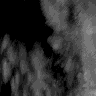
\includegraphics[width=\linewidth]{fig/radarcs1801030500.png}
	    \end{subfigure}
	    % ---------------
	    \begin{subfigure}{.3\textwidth}
	        \centering
	        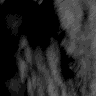
\includegraphics[width=\linewidth]{fig/radarcs1801030510.png}
	    \end{subfigure}
	    % ---------------
	    \begin{subfigure}{.3\textwidth}
	        \centering
	        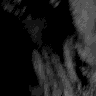
\includegraphics[width=\linewidth]{fig/radarcs1801030520.png}
	    \end{subfigure}
	\end{figure}

	\begin{figure}
	    % ---------------
	    \begin{subfigure}{.3\textwidth}
	        \centering
	        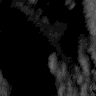
\includegraphics[width=\linewidth]{fig/radarcs1801030530.png}
	    \end{subfigure}
	    % ---------------
	    \begin{subfigure}{.3\textwidth}
	        \centering
	        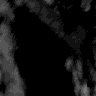
\includegraphics[width=\linewidth]{fig/radarcs1801030540.png}
	    \end{subfigure}
	    % ---------------
	    \begin{subfigure}{.3\textwidth}
	        \centering
	        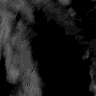
\includegraphics[width=\linewidth]{fig/radarcs1801030550.png}
	    \end{subfigure}
	\end{figure}
\end{frame}

% -----------------------------------------------
\section{Weather Radar Images}

\begin{frame}{}
	\begin{figure}
		\centering
		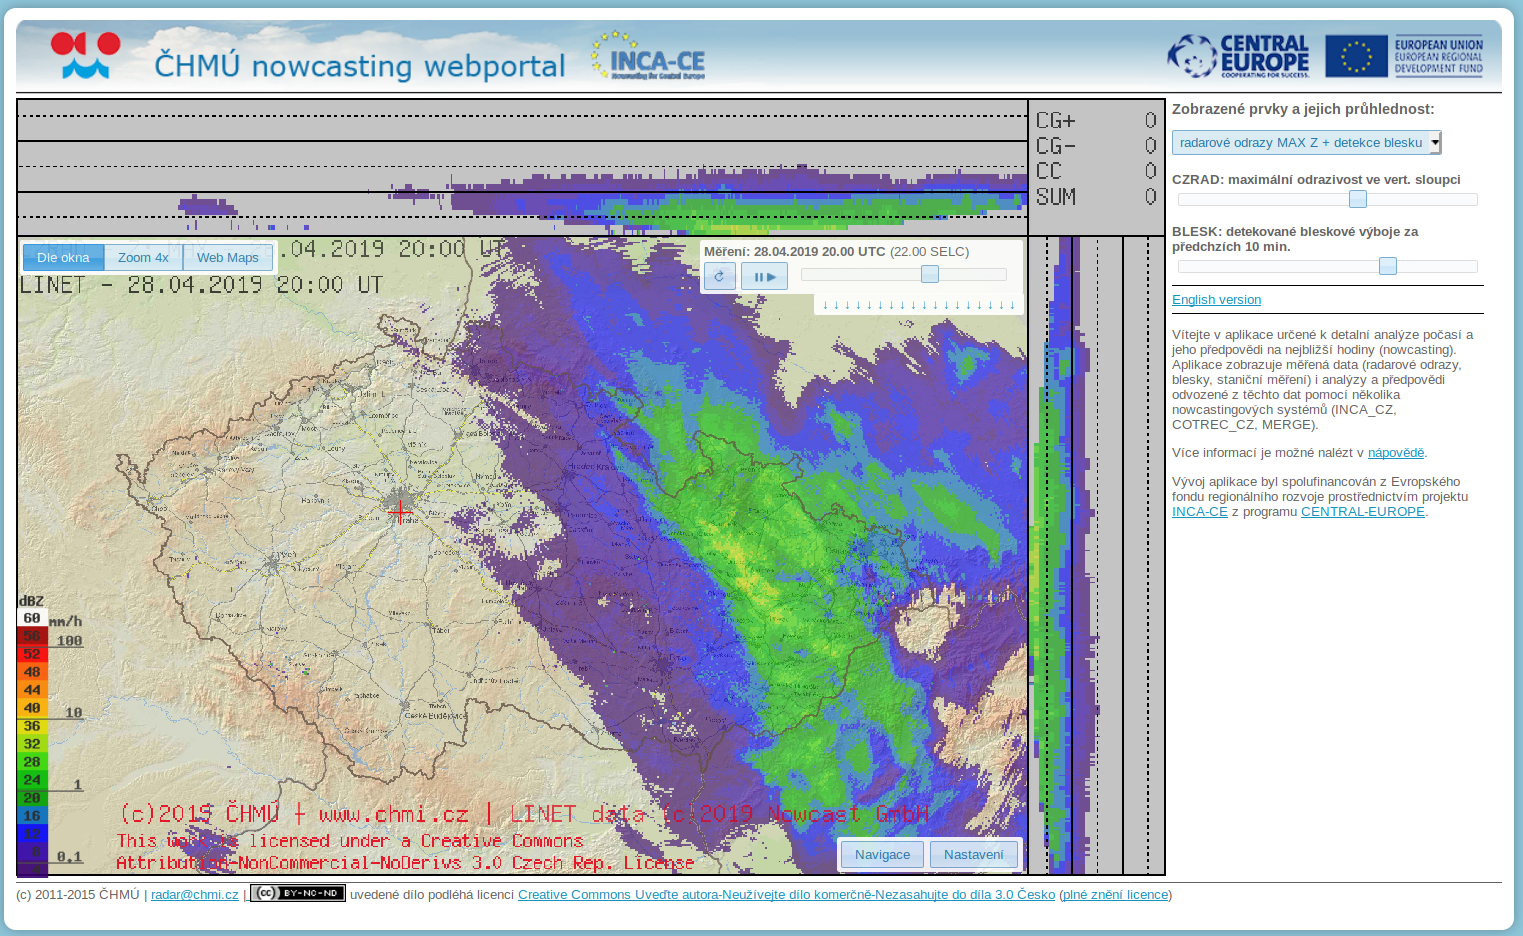
\includegraphics[width=\linewidth]{fig/01_czrad_portal.png}
	\end{figure}

	\footnotesize Screenshot of the CHMI radar images from the nowcasting webportal at\\ \url{portal.chmi.cz/files/portal/docs/meteo/rad/inca-cz/short.html}
	\normalsize
\end{frame}

\begin{frame}{}
	\begin{figure}
	    % ---------------
	    % 582 * 296
	    % ---------------
	    \begin{subfigure}{.48\linewidth}
	        \centering
	        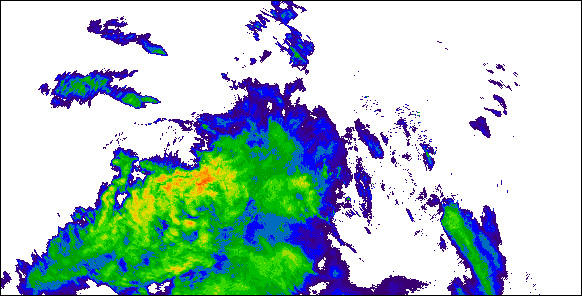
\includegraphics[width=\linewidth]{fig/04_czrad_colour.png}
	    \end{subfigure}
	    % ---------------
	    \begin{subfigure}{.48\linewidth}
	        \centering
	        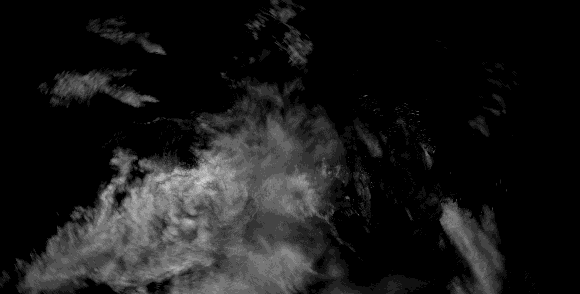
\includegraphics[width=\linewidth]{fig/04_czrad_gray.png}
	    \end{subfigure}
	    % ---------------
	\end{figure}

	\begin{figure}
	    \centering
	    \begin{minipage}{.8\linewidth}
	        \begin{mdframed}[style=MyFrame,nobreak=true,align=center,userdefinedwidth=.8\linewidth]
	            
\includegraphics[width=\linewidth]{fig/04_colourspace.png}
	        \end{mdframed}
	    \end{minipage}
	\end{figure}

	\pause

	\begin{figure}
	    \centering
	    \begin{minipage}{.35\linewidth}
	        \centering
	        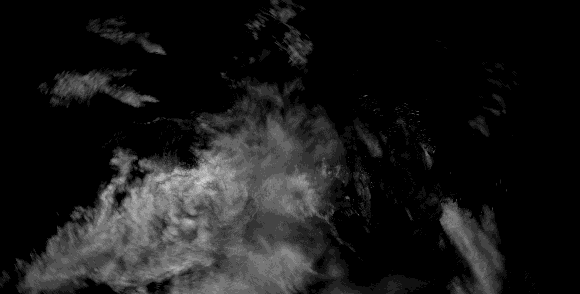
\includegraphics[height=0.17\textheight]{fig/04_czrad_gray.png}
	    \end{minipage}%
	    $\rightarrow$
	    \begin{minipage}{0.25\linewidth}
	        \centering
	        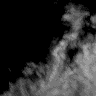
\includegraphics[height=0.17\textheight]{fig/crop/34.png}
	    \end{minipage}
	    \begin{minipage}{0.25\linewidth}
	        \centering
	        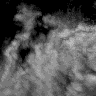
\includegraphics[height=0.17\textheight]{fig/crop/35.png}
	    \end{minipage}
	\end{figure}
\end{frame}

% -----------------------------------------------

\begin{frame}{}
	\begin{figure}
		\centering
		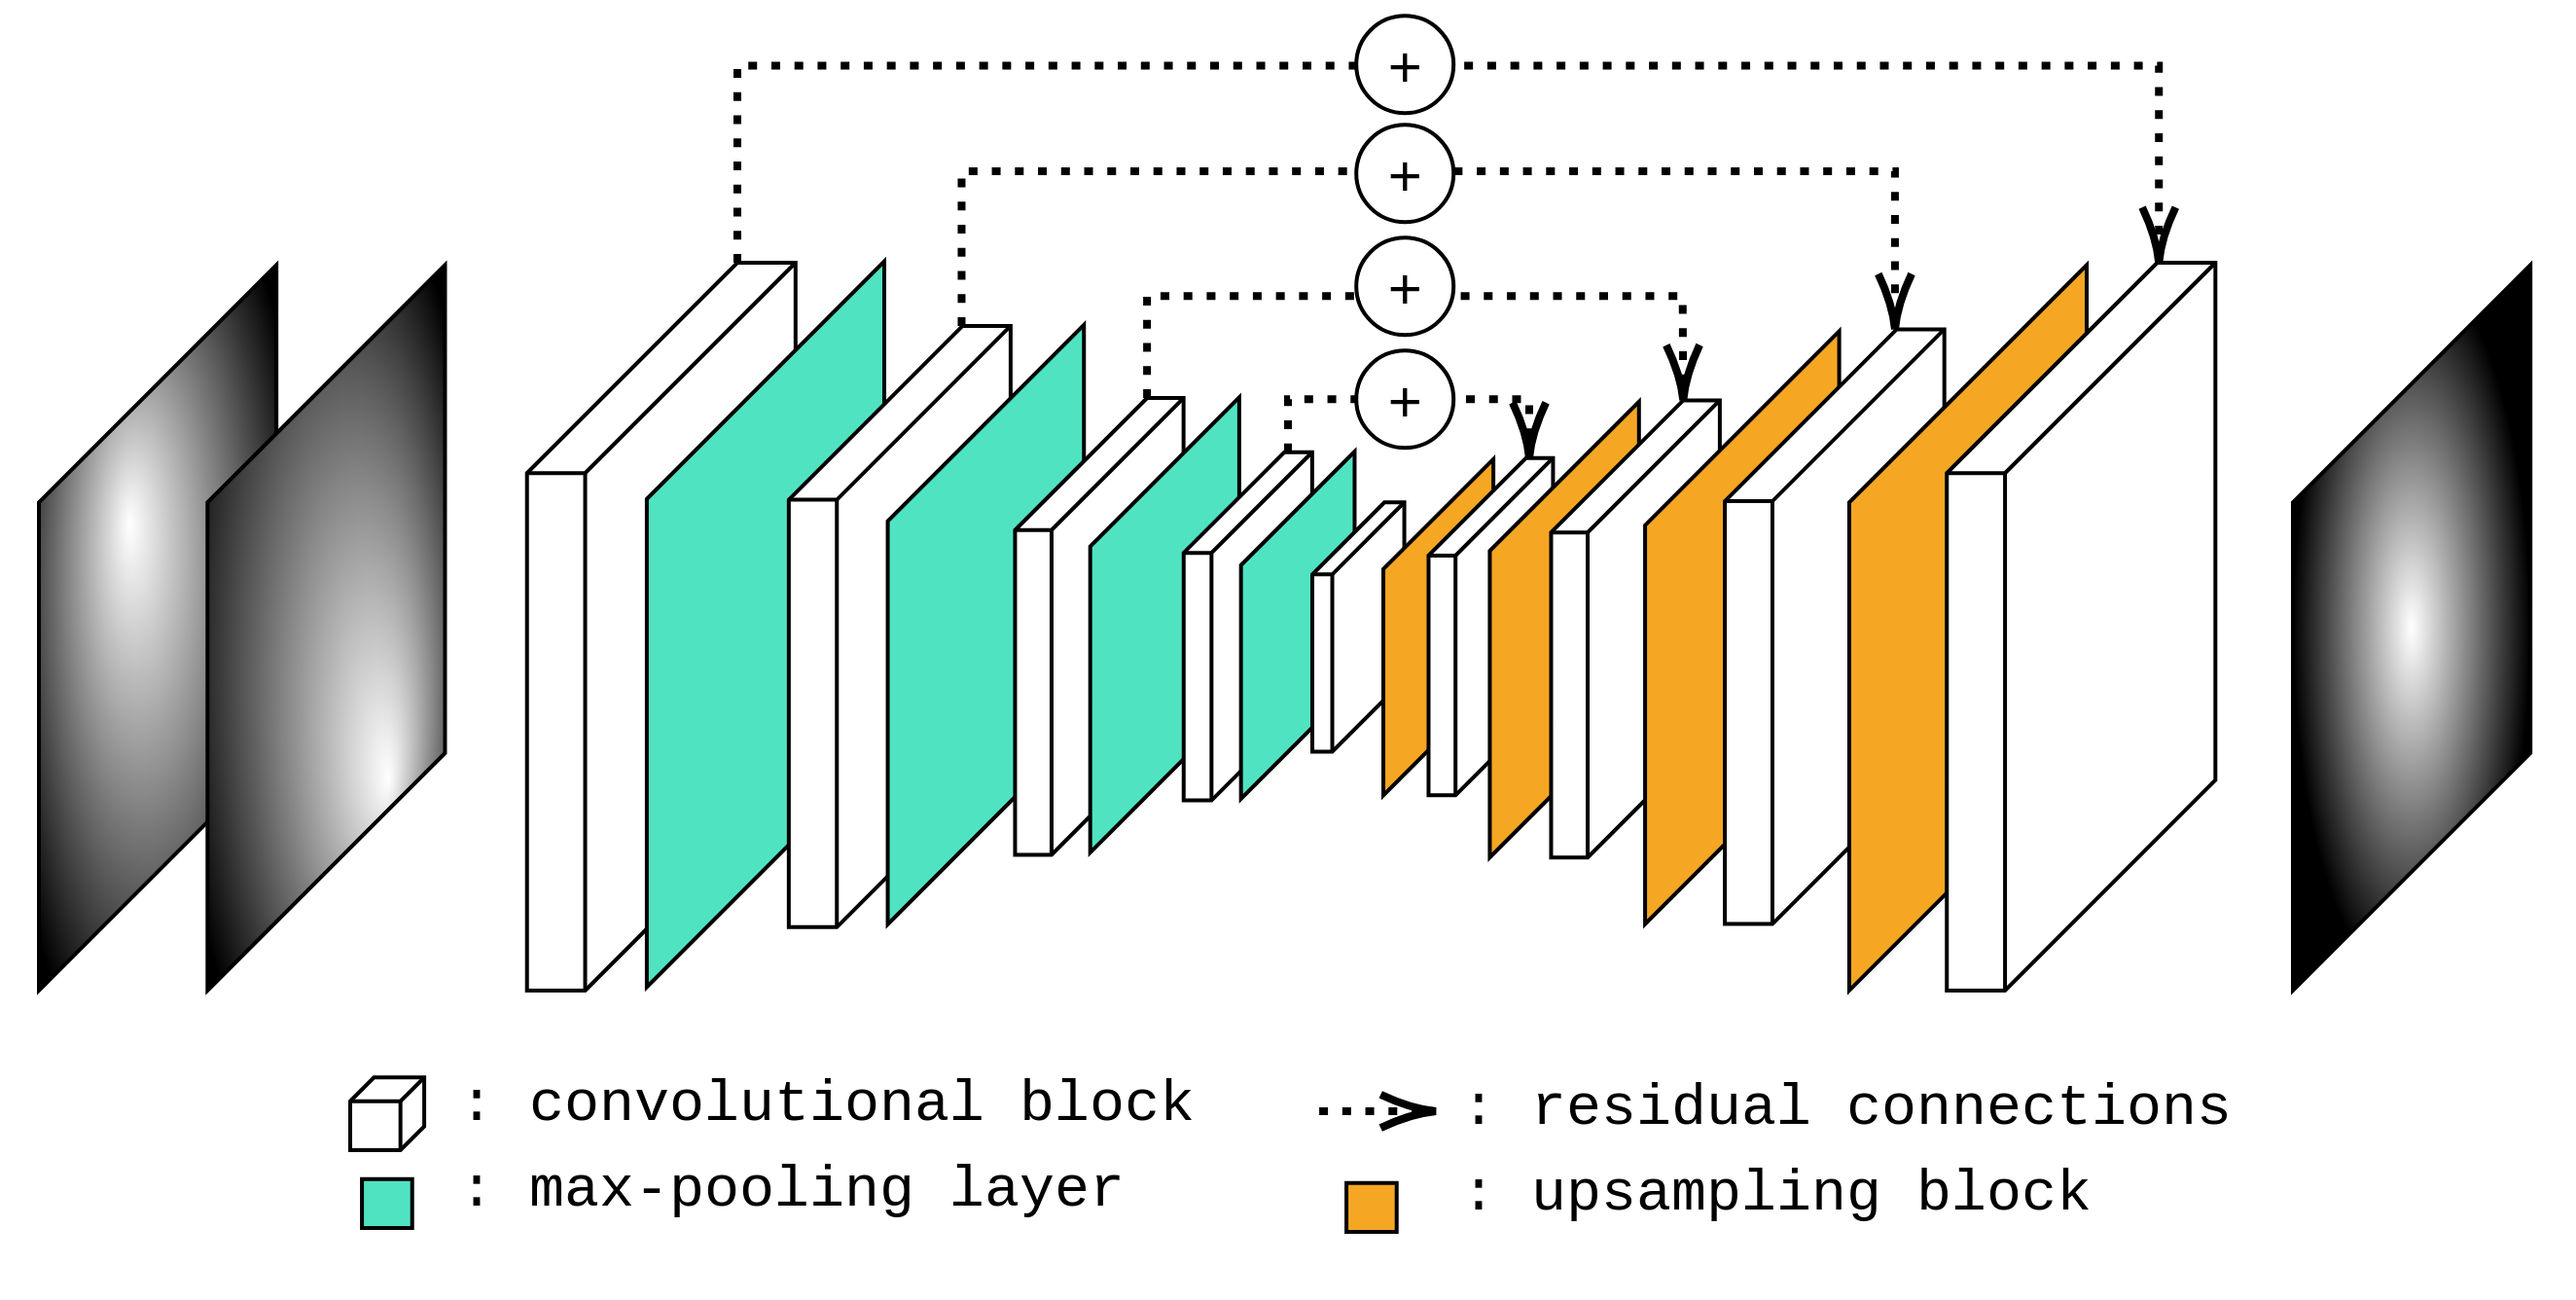
\includegraphics[width=\linewidth]{fig/05_cnn_arch.png}
	\end{figure}
\end{frame}


% -----------------------------------------------
\begin{frame}{Interpolation Results}
	\begin{figure}
	    % ---------------
	    \begin{subfigure}{.3\textwidth}
	        \centering
	        \begin{mdframed}[style=blue,nobreak=true,align=center]
	        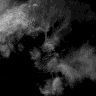
\includegraphics[width=\linewidth]{fig/inter/0.png}
	        \end{mdframed}
	    \end{subfigure}
	    % ---------------
	    \begin{subfigure}{.3\textwidth}
	        \centering
	        \begin{mdframed}[style=red,nobreak=true,align=center]
	        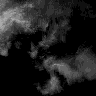
\includegraphics[width=\linewidth]{fig/inter/1.png}
	        \end{mdframed}
	    \end{subfigure}
	    % ---------------
	    \begin{subfigure}{.3\textwidth}
	        \centering
	        \begin{mdframed}[style=blue,nobreak=true,align=center]
	        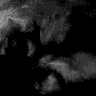
\includegraphics[width=\linewidth]{fig/inter/3.png}
	        \end{mdframed}
	    \end{subfigure}
	\end{figure}

	\begin{figure}
	    % ---------------
	    \begin{subfigure}{.3\textwidth}
	        \centering
	        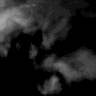
\includegraphics[width=\linewidth]{fig/inter/2.png}
	    \end{subfigure}
	    % ---------------
	\end{figure}
\end{frame}

% -----------------------------------------------
\begin{frame}{Interpolation Results}
	\begin{figure}
	    % ---------------
	    \begin{subfigure}{.48\linewidth}
	        \centering
	        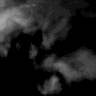
\includegraphics[width=\linewidth]{fig/inter/2.png}
	        \caption{Predicted.}
	    \end{subfigure}
	    % ---------------
	    \begin{subfigure}{.48\linewidth}
	        \centering
	        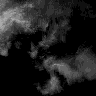
\includegraphics[width=\linewidth]{fig/inter/1.png}
	        \caption{Ground truth.}
	    \end{subfigure}
	    % ---------------
	\end{figure}
\end{frame}
% =========================================================================
\begin{frame}{Extrapolation}
	\begin{figure}
	    % ---------------
	    \begin{subfigure}{.3\textwidth}
	        \centering
	        \begin{mdframed}[style=blue,nobreak=true,align=center]
	        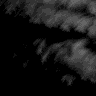
\includegraphics[width=\linewidth]{fig/extra/0.png}
	        \end{mdframed}
	    \end{subfigure}
	    % ---------------
	    \begin{subfigure}{.3\textwidth}
	        \centering
	        \begin{mdframed}[style=blue,nobreak=true,align=center]
	        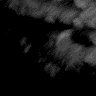
\includegraphics[width=\linewidth]{fig/extra/1.png}
	        \end{mdframed}
	    \end{subfigure}
	    % ---------------
	    \begin{subfigure}{.3\textwidth}
	        \centering
	        \begin{mdframed}[style=blue,nobreak=true,align=center]
	        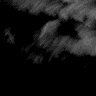
\includegraphics[width=\linewidth]{fig/extra/2.png}
	        \end{mdframed}
	    \end{subfigure}
	\end{figure}

	\begin{figure}
	    % ---------------
	    \begin{subfigure}{.3\textwidth}
	        \centering
	        \begin{mdframed}[style=red,nobreak=true,align=center]
	        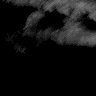
\includegraphics[width=\linewidth]{fig/extra/3.png}
	        \end{mdframed}
	    \end{subfigure}
	    % ---------------
	    \begin{subfigure}{.3\textwidth}
	        \centering
	        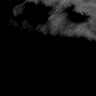
\includegraphics[width=\linewidth]{fig/extra/4.png}
	    \end{subfigure}
	    % ---------------
	    \begin{subfigure}{.3\textwidth}
	        \centering
	        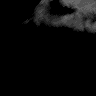
\includegraphics[width=\linewidth]{fig/extra/5.png}
	    \end{subfigure}
	\end{figure}
\end{frame}

\begin{frame}{Extrapolation}
	\begin{figure}
	    % ---------------
	    \begin{subfigure}{.3\textwidth}
	        \centering
	        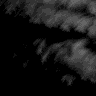
\includegraphics[width=\linewidth]{fig/extra/0.png}
	    \end{subfigure}
	    % ---------------
	    \begin{subfigure}{.3\textwidth}
	        \centering
	        \begin{mdframed}[style=blue,nobreak=true,align=center]
	        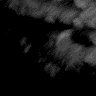
\includegraphics[width=\linewidth]{fig/extra/1.png}
	        \end{mdframed}
	    \end{subfigure}
	    % ---------------
	    \begin{subfigure}{.3\textwidth}
	        \centering
	        \begin{mdframed}[style=blue,nobreak=true,align=center]
	        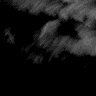
\includegraphics[width=\linewidth]{fig/extra/2.png}
	        \end{mdframed}
	    \end{subfigure}
	\end{figure}

	\begin{figure}
	    % ---------------
	    \begin{subfigure}{.3\textwidth}
	        \centering
	        \begin{mdframed}[style=blue,nobreak=true,align=center]
	        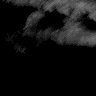
\includegraphics[width=\linewidth]{fig/extra/3.png}
	        \end{mdframed}
	    \end{subfigure}
	    % ---------------
	    \begin{subfigure}{.3\textwidth}
	        \centering
	        \begin{mdframed}[style=red,nobreak=true,align=center]
	        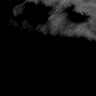
\includegraphics[width=\linewidth]{fig/extra/4.png}
	        \end{mdframed}
	    \end{subfigure}
	    % ---------------
	    \begin{subfigure}{.3\textwidth}
	        \centering
	        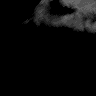
\includegraphics[width=\linewidth]{fig/extra/5.png}
	    \end{subfigure}
	\end{figure}
\end{frame}

\begin{frame}{Extrapolation - Results}
	\begin{figure}
	    % ---------------
	    \begin{subfigure}{.3\textwidth}
	        \centering
	        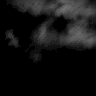
\includegraphics[width=\linewidth]{fig/extra/out_0.png}
	    \end{subfigure}
	    % ---------------
	    \begin{subfigure}{.3\textwidth}
	        \centering
	        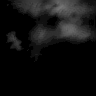
\includegraphics[width=\linewidth]{fig/extra/out_1.png}
	    \end{subfigure}
	    % ---------------
	    \begin{subfigure}{.3\textwidth}
	        \centering
	        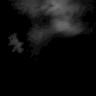
\includegraphics[width=\linewidth]{fig/extra/out_2.png}
	    \end{subfigure}
	    \caption{Predicted sequence.}
	\end{figure}

	\begin{figure}
	    % ---------------
	    \begin{subfigure}{.3\textwidth}
	        \centering
	        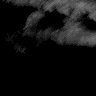
\includegraphics[width=\linewidth]{fig/extra/3.png}
	    \end{subfigure}
	    % ---------------
	    \begin{subfigure}{.3\textwidth}
	        \centering
	        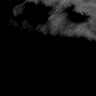
\includegraphics[width=\linewidth]{fig/extra/4.png}
	    \end{subfigure}
	    % ---------------
	    \begin{subfigure}{.3\textwidth}
	        \centering
	        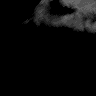
\includegraphics[width=\linewidth]{fig/extra/5.png}
	    \end{subfigure}
	    \caption{Ground truth sequence.}
	\end{figure}
\end{frame}

\begin{frame}{Extrapolation - Results}
	\begin{figure}
	    % ---------------
	    \begin{subfigure}{.48\linewidth}
	        \centering
	        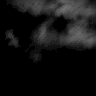
\includegraphics[width=\linewidth]{fig/extra/out_0.png}
	        \caption{Predicted.}
	    \end{subfigure}
	    % ---------------
	    \begin{subfigure}{.48\linewidth}
	        \centering
	        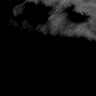
\includegraphics[width=\linewidth]{fig/extra/4.png}
	        \caption{Ground truth.}
	    \end{subfigure}
	    % ---------------
	\end{figure}
\end{frame}
% -----------------------------------------------
\begin{frame}
\centering \LARGE
	Thank you for your attention!

% \vskip 2cm

% \tiny
% 	\begin{block}{References}
% 	\renewcommand*{\bibfont}{\tiny}
% 	\nocite{2016arXiv160605908D}
% 	\nocite{VAE_lecture}
% 	\nocite{Autoencoders}
% 	\printbibliography
% 	\end{block}

\end{frame}



% -------------------------------------------------------------------------------------------------
% -------------------------------------------------------------------------------------------------
% -------------------------------------------------------------------------------------------------

% \section{Introduction}

% \begin{frame}{Introduction}

% \begin{itemize}
%   \item Your introduction goes here!
%   \item Use \texttt{itemize} to organize your main points.
% \end{itemize}

% \vskip 1cm

% \begin{block}{Examples}
% Some examples of commonly used commands and features are included, to help you get started.
% \end{block}

% \end{frame}

% \section{Some \LaTeX{} Examples}

% \subsection{Tables and Figures}

% \begin{frame}{Tables and Figures}

% \begin{itemize}
% \item Use \texttt{tabular} for basic tables --- see Table~\ref{tab:widgets}, for example.
% \item You can upload a figure (JPEG, PNG or PDF) using the files menu. 
% \item To include it in your document, use the \texttt{includegraphics} command (see the comment below in the source code).
% \end{itemize}

% % Commands to include a figure:
% %\begin{figure}
% %\includegraphics[width=\textwidth]{your-figure's-file-name}
% %\caption{\label{fig:your-figure}Caption goes here.}
% %\end{figure}

% \begin{table}
% \centering
% \begin{tabular}{l|r}
% Item & Quantity \\\hline
% Widgets & 42 \\
% Gadgets & 13
% \end{tabular}
% \caption{\label{tab:widgets}An example table.}
% \end{table}

% \end{frame}

% \subsection{Mathematics}

% \begin{frame}{Readable Mathematics}

% Let $X_1, X_2, \ldots, X_n$ be a sequence of independent and identically distributed random variables with $\text{E}[X_i] = \mu$ and $\text{Var}[X_i] = \sigma^2 < \infty$, and let
% $$S_n = \frac{X_1 + X_2 + \cdots + X_n}{n}
%       = \frac{1}{n}\sum_{i}^{n} X_i$$
% denote their mean. Then as $n$ approaches infinity, the random variables $\sqrt{n}(S_n - \mu)$ converge in distribution to a normal $\mathcal{N}(0, \sigma^2)$.

% \end{frame}

\end{document}